\subsection{Screen}
Beim Starten der App erscheint (sofern eine WLan-Verbindung aktiv ist) die in 
\ref{fig:startScreen} dargestellte Benutzerschnittstelle.\\
Ist der QR-Code korrekt, so kommt die HMI der App zum Vorschein. Hierbei 
startet als erstes immer der Tab, in dem die Maschinendaten dargestellt werden 
(s. \ref{fig:tabMachineData}).
\newpage
% ------------------------------
% Bild einfügen
% ------------------------------
\begin{figure}[H]
	\centering
	\fbox{	\includegraphics[width=0.85\textwidth]{03_Grafiken/startScreen.jpg}}
	\caption[Startscreen]{Startscreen}
	\label{fig:startScreen}
\end{figure}

% ------------------------------
% Bild einfügen
% ------------------------------
\begin{figure}[H]
	\centering
	\fbox{	
	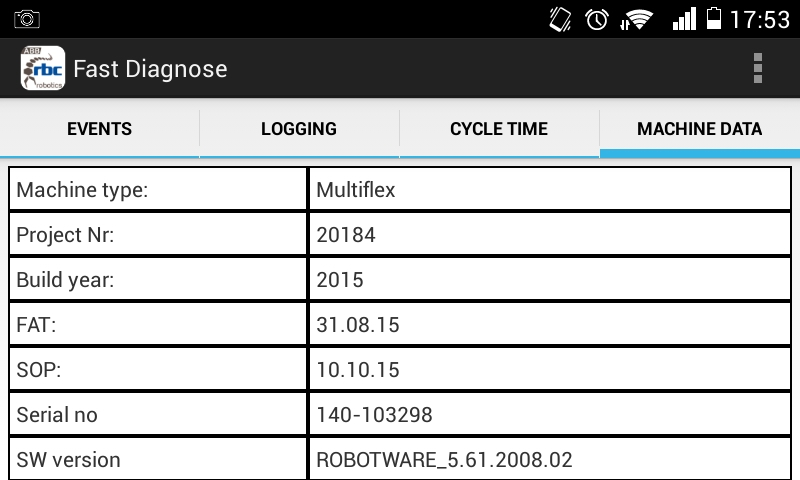
\includegraphics[width=0.85\textwidth]{03_Grafiken/tabMachineData.jpeg}}
	\caption[Tab Machine Data]{Tab Machine Data}
	\label{fig:tabMachineData}
\end{figure}

Das Erscheinungsbild aller weiteren Tabs ist in \ref{fig:tabEvents}, 
\ref{fig:tabLogging} und \ref{fig:tabCycleTime} dargestellt.

% ------------------------------
% Bild einfügen
% ------------------------------
\begin{figure}[H]
	\centering
	\fbox{	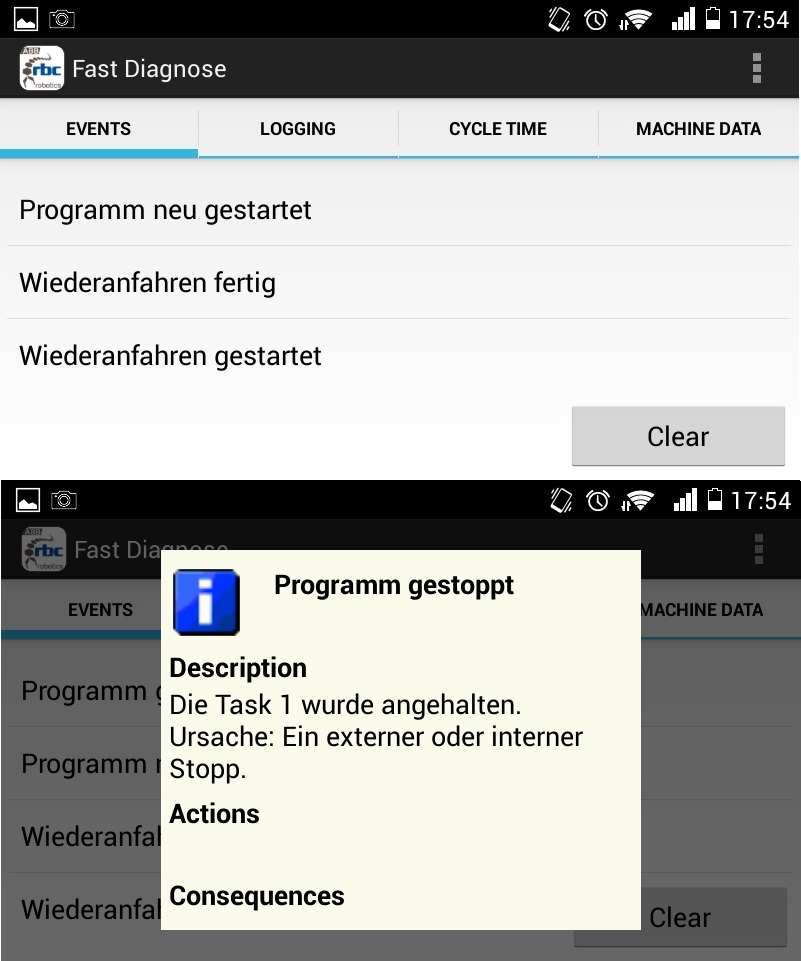
\includegraphics[width=0.85\textwidth]{03_Grafiken/tabEvents.jpeg}}
	\caption[Tab Events]{Tab Events (o: Event-Liste, u: Event-Dialog)}
	\label{fig:tabEvents}
\end{figure}

% ------------------------------
% Bild einfügen
% ------------------------------
\begin{figure}[H]
	\centering
		\fbox{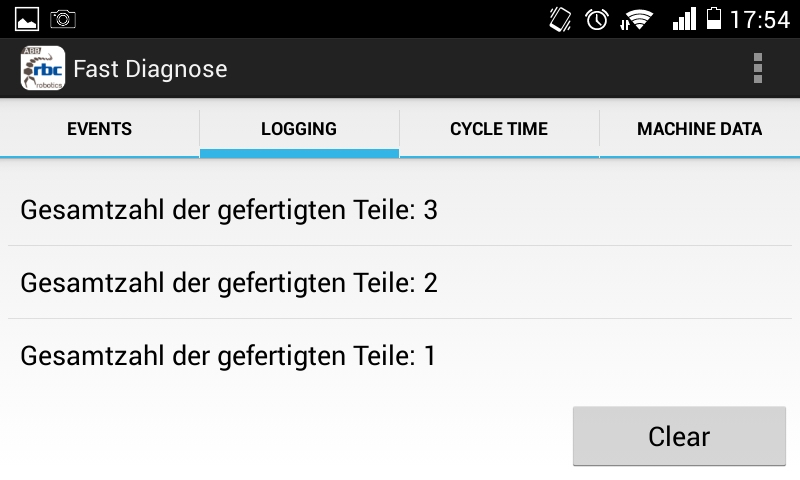
\includegraphics[width=0.85\textwidth]{03_Grafiken/tabLogging.jpeg}}
	\caption[Tab Logging]{Tab Logging}
	\label{fig:tabLogging}
\end{figure}

% ------------------------------
% Bild einfügen
% ------------------------------
\begin{figure}[H]
	\centering
		\fbox{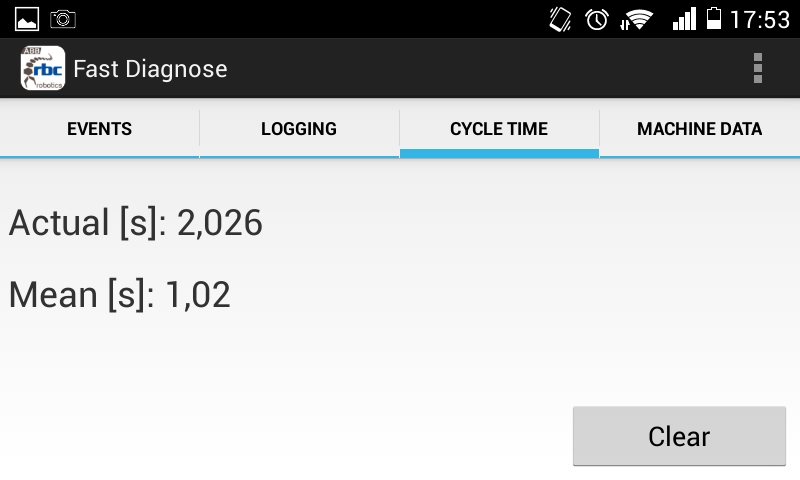
\includegraphics[width=0.85\textwidth]{03_Grafiken/tabCycleTime.jpeg}}
	\caption[Tab Cycle Time]{Tab Cycle Time}
	\label{fig:tabCycleTime}
\end{figure}